% This is a LaTeX tutorial by Overleaf titled [Free online introduction to LaTeX (part 3)](https://www.overleaf.com/learn/latex/Free_online_introduction_to_LaTeX_(part_3)).

\documentclass{beamer}
\usepackage{graphicx}

%\usetheme{Darmstadt}
%\usecolortheme{beetle}

\title{This is my slide!!!}
\author{Tran Phong Binh}
\institute{National Tsing Hua University}
\date{\today}

\begin{document}

\begin{frame}
    \titlepage
\end{frame}

\begin{frame}
    \frametitle{Table of Contents}
    \tableofcontents
\end{frame}

\section{First section}
\begin{frame}
    \frametitle{This is the first slide of the first section baby!}
    \begin{itemize}
        \item Use \texttt{frametitle} to give the frame a title.
        \item Then add content to the frame.
        \item The source for this frame looks like \ldots
    \end{itemize}
\end{frame}

\section{Second section}
\begin{frame}
    \frametitle{First slide of the second section!!}
    \tableofcontents[currentsection]
\end{frame}

\begin{frame}
    \frametitle{Use of \texttt{column}s mate!!}
    \begin{columns}
        \begin{column}{0.4\textwidth}
            \begin{itemize}
                \item I should \emph{emphasize} that this is an \alert{important} point.
                \item The argument \ldots
                \item See also the \ldots
            \end{itemize}
        \end{column}
        \begin{column}{0.6\textwidth} % 20210614 0.4 + 0.6 = 1? any other possibilities?
        Second column's content here bitch.
        \end{column}
    \end{columns}
\end{frame}

\begin{frame}
    \frametitle{Add some sexy pictures baby.}
    \begin{figure}
        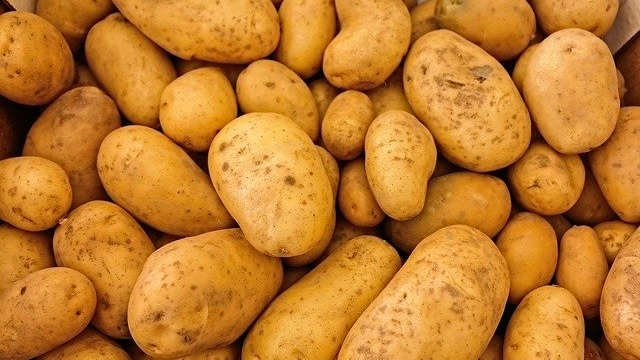
\includegraphics[width=0.5\textwidth]{potato}
    \end{figure}
\end{frame}

\begin{frame}
    \frametitle{Wanna add tables?}
    \begin{table}
        \begin{tabular}{ |l|r|r| }
            \hline
            Item & Qty & Unit \$ \\
            \hline
            Widget & 1 & 199.99 \\
            Gadget & 2 & 399.99 \\
            Cable & 3 & 19.99 \\
            \hline
        \end{tabular}
        \caption{An ordinary table.}
    \end{table}
\end{frame}

\begin{frame}
    \frametitle{Use of \texttt{block}s bae.}
    \begin{block}{Interesting Fact}
    This is important.
    \end{block}
    \begin{alertblock}{Caution}
    This is really important!
    \end{alertblock}
\end{frame}

\begin{frame}
    \begin{itemize}
        \item Can you feel the
        \pause \item anticipation?
    \end{itemize}
\end{frame}

\end{document}